\documentclass[hyperref=unicode]{beamer}

\usepackage[absolute,overlay]{textpos}
\usepackage{graphicx}
\usepackage{adjustbox}
\usepackage{chemfig}
\usepackage[version=4]{mhchem}
\usepackage{wrapfig}
\usepackage{multirow}
\adjustboxset*{center}
\usepackage{caption}
\usepackage{chemformula}
\usepackage{elements}

%dělení slov
\usepackage{ragged2e}
\let\raggedright=\RaggedRight
%konec dělení slov

\usepackage{fontspec}
\usepackage{unicode-math}

\usepackage{polyglossia}
\setdefaultlanguage{czech}

\def\uv#1{„#1“}

\mode<presentation>{\usetheme{Madrid}}
\DefineNamedColor{named}{pozadi}{RGB}{200,200,200}
\usecolortheme{crane}

\setbeamertemplate{footline}[frame number]

\addtobeamertemplate{frametitle}{
	\let\insertframetitle\insertsectionhead}{}
\addtobeamertemplate{frametitle}{
	\let\insertframesubtitle\insertsubsectionhead}{}

\makeatletter
\CheckCommand*\beamer@checkframetitle{\@ifnextchar\bgroup\beamer@inlineframetitle{}}
\renewcommand*\beamer@checkframetitle{\global\let\beamer@frametitle\relax\@ifnextchar\bgroup\beamer@inlineframetitle{}}
\makeatother
\setbeamercolor{section in toc}{fg=blue}
\setbeamertemplate{section in toc shaded}[default][100]

\title[Crisis] % (optional, only for long titles)
{Infračervená spektroskopie}

\author % (optional, for multiple authors)
{Zdeněk Moravec, C12/316, hugo@chemi.muni.cz}

\date{} %hide date on titlepage

\subtitle{C5060 Metody chemické výzkumu}

\begin{document}
\frame{\titlepage}

\section{Osnova}
\frame{
	\frametitle{}
	\vfill
	\begin{itemize}
	\item Molekulová spektroskopie
	\item Základní principy IR spektroskopie
	\item Symetrie molekul
	\item Měřící techniky
	\begin{itemize}
		\item FT-IR transmisní měření
		\item ATR, DRIFTS, PAS
		\item TG/IR, GC/IR
	\end{itemize}
	\end{itemize}
	\vfill
}

\section{Molekulová spektroskopie}
\frame{
	\frametitle{}
	\vfill
	\begin{itemize}
	\item Studuje interakci elektromagnetického záření s~molekulami vzorku
	\item Jde o kvalitativní i kvantitativní analytickou metodu
	\item Metody molekulové spektroskopie
	\begin{itemize}
		\item Infračervená spektroskopie
		\item Ramanova spektroskopie
		\item Mikrovlnná spektroskopie
	\end{itemize}
	\end{itemize}
	\vfill
}

\frame{
	\frametitle{}
	\vfill
	\begin{itemize}
	\item Soubor metod založených na využití těch vlastností molekul, které jsou spojeny s přítomností:
	\begin{itemize}
		\item kovalentních vazeb
		\item koordinačních vazeb
	\end{itemize}
	\end{itemize}
	\begin{center}
	$\chemfig{H-\charge{0=\:}{N}(-[:60]H)(-[:300]H)}$
	\hspace{40mm}
	$\chemfig{F-B(-[:60]F)(-[:300]F)}$
	$\chemfig{F-B(-[:120]F)(-[:240]F)(-N(-[:60]H)(-[:0]H)(-[:300]H))}$
	\end{center}
	\vfill
}

\section{Elektromagnetické záření}
\frame{
	\frametitle{}
	\vfill
	\begin{itemize}
	\item Kombinace magnetického a elektrického vlnění (pole)
	\item $E = h.f = \frac{hc}{\lambda} = hc \tilde{\nu}$
	\begin{itemize}
		\item E - energie záření
		\item h - Planckova konstanta: $6,626 176(36).10^{-34}$ Js
		\item f - frekvence záření
		\item c - rychlost světla: $2,997 924 58(01).10^8$ m.s$^{-1}$
		\item $\lambda$ - vlnová délka
		\item $\tilde{\nu}$ - vlnočet
	\end{itemize}
	\end{itemize}
	\begin{figure}
		\adjincludegraphics[width=.8\textwidth]{../img/elmag.png}
		\caption*{Složky elektromagnetického záření.\footnote[frame]{Zdroj: \href{https://commons.wikimedia.org/wiki/File:Onde_electromagnetique.svg}{SuperManu/Commons}}}
	\end{figure}
	\vfill
}

\subsection{Vlnová délka, frekvence, vlnočet, energie}
\frame{
	\frametitle{}
	\vfill
	\begin{itemize}
	\item \emph{Vlnová délka} ($\lambda$) - dráha, kterou urazí vlna během jednoho kmitu. $1 \textrm{\r{A}} = 10^{-10}$ m = 0,1 nm
	\item \emph{Frekvence} (f) - počet kmitů vlny za 1 s. 1 Hz = 1 $\textrm{s}^{-1}$
	\item \emph{Vlnočet} ($\tilde{\nu}$) - počet vln, připadající na dráhu 1 cm ve směru šíření vlny [cm$^{-1}$]
	\item $E = h.f = \frac{hc}{\lambda} = hc \tilde{\nu}$
	\end{itemize}

	\begin{figure}
		\adjincludegraphics[width=.8\textwidth]{../img/elmag.png}
		\caption*{Složky elektromagnetického záření.\footnote[frame]{Zdroj: \href{https://commons.wikimedia.org/wiki/File:Onde_electromagnetique.svg}{SuperManu/Commons}}}
	\end{figure}
	\vfill
}

\subsection{Spektrum elektromagnetického záření}
\frame{
	\frametitle{}
	\vfill
	\begin{figure}
		\adjincludegraphics[width=.8\textwidth]{../img/elmag-spek.png}
		\caption*{Elektromagnetické spektrum.\footnote[frame]{Zdroj: \href{https://commons.wikimedia.org/wiki/File:EM_Spectrum_Properties_edit.svg}{Inductiveload, NASA/Commons}}}
	\end{figure}
	\vfill
}

\frame{
	\frametitle{}
	\vfill
	\begin{tabular}{|p{2.2cm}|p{3cm}|p{2cm}|p{2cm}|}
	\hline
	& UV-VIS & IR & MW \\
	& 50-800 nm & 1-100 $\mu$m & 1-10 mm \\
	\hline
	Elektronická
	\newline spektroskopie & Absorpční UV-VIS
	\newline Luminiscenční spektroskopie & & \\
	\hline
	Vibrační
	\newline spektroskopie & Ramanova spektroskopie & Infračervená spektroskopie & \\
	\hline
	Rotační
	\newline spektroskopie & Ramanova spektroskopie & & Mikrovlnná spektroskopie \\
	\hline
	\end{tabular}
	\vfill
}

\section{Základní principy IR spektroskopie}
\subsection{Vibrace chemických vazeb}
\frame{
	\frametitle{}
	\vfill
	\begin{itemize}
	\item Během vibrace vazby dochází k přechodu systému na jinou energetickou hladinu.
	\item Energie (frekvence) vibrace závisí na síle vazby a hmotnosti atomů, které vazbu tvoří.
	\item $\nu = \frac{1}{2\pi}\sqrt{\frac{k}{\mu}}; \mu = \frac{m_1m_2}{m_1 + m_2}$
	\item $\nu$ - frekvence vibrace; k - silová konstanta; $\mu$ - redukovaná hmotnost; m$_1$,m$_2$ - hmotnosti atomů
	\item \textit{Silová konstanta vazby} (k) - závisí na hmotnosti atomů, vazebné energii a řádu vazby.
	\item \textit{Redukovaná hmotnost} ($\mu$) - umožňuje řešit fyzikální \textit{problém dvou těles}, jako by se jednalo o těleso jedno.\footnotemark
	\end{itemize}
	\begin{center}
		\adjincludegraphics[width=3cm]{../img/oscillator.png}
	\end{center}
	\vfill
	\footnotetext[1]{\href{https://scienceworld.wolfram.com/physics/Two-BodyProblem.html}{Two-Body Problem}}
}

\frame{
	\frametitle{}
	\vfill
	\begin{itemize}
	\item Přechod mezi základní a 1. excitovanou hladinou se nazývá \emph{základní (fundamentální) vibrace}.
	\item Pokud dochází k přechodům na vyšší hladinu, jedná se o tzv. \emph{vyšší harmonické přechody (overtony)}. Jejich frekvence jsou \em přibližně \em násobkem fundamentální frekvence (energetické hladiny se postupně zhušťují).
	\item Pokud dojde k současné změně dvou vibračních stav molekuly jedná se o \emph{kombinační přechody}.
	\item \textbf{Valenční vibrace} – dochází ke změně mezijaderné vzdálenosti.
	\item \textbf{Deformační vibrace} – dochází ke změně vazebného úhlu.
	\end{itemize}
	\vfill
}

\subsection{Vibrace ve víceatomové molekule}
\frame{
	\frametitle{}
	\vfill
	\begin{itemize}
	\item Víceatomové molekuly můžeme popsat jako soustavy hmotných bodů.
	\item Výsledná vibrace je rovna součtu normálních vibrací.
	\item Počet normálních vibrací je roven počtu vibračních stupňů volnosti. Pro nelineární  molekulu o N atomech je počet vibrací roven 3N-6, u lineární je to 3N-5.
	\end{itemize}
	\vfill
}

\subsection{Vibrace v lineární  molekule}
\frame{
	\frametitle{}
	\vfill
	\begin{itemize}
	\item Lineární molekula -- \ce{CO2} -- N = 3
	\item 3N-5 = 3x3-5 = 4
	\end{itemize}
	\begin{figure}
		
\includegraphics[width=.8\textwidth]{../img/CO2.png}
	\end{figure}
	\vfill
}

\subsection{Vibrace v nelineární  molekule}
\frame{
	\frametitle{}
	\vfill
	\begin{itemize}
	\item Nelineární molekula -- \ce{H2O} -- N = 3
	\item 3N-6 = 3x3-6 = 3
	\end{itemize}
	\begin{figure}
		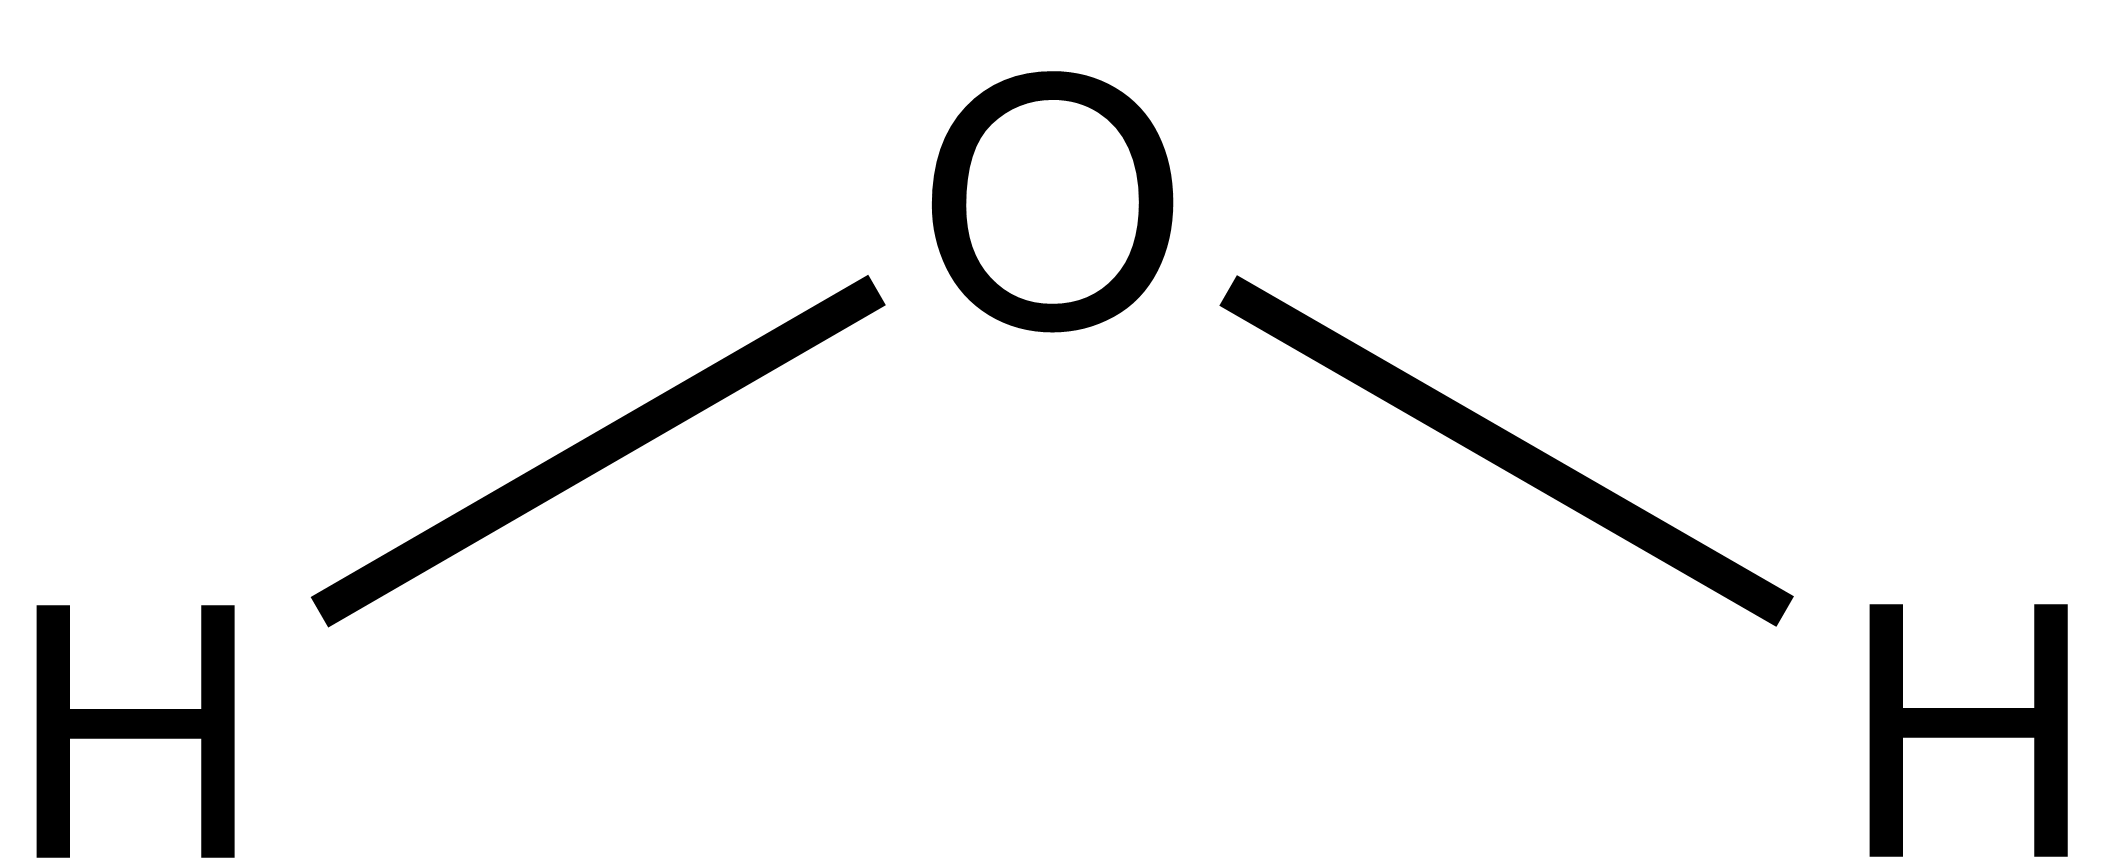
\includegraphics[width=.8\textwidth]{../img/water-struct.png}
	\end{figure}
	\vfill
}

\subsection{Symetrie molekul}
\frame{
	\frametitle{}
	\vfill
	\begin{itemize}
	\item Struktura a symetrie molekuly je velmi důležitá pro interpretaci molekulových spekter.
	\item \textbf{Operace symetrie} - geometrická operace, jejímž provedením dostaneme objekt do polohy nerozlišitelné od výchozí.
	\item \textbf{Prvek symetrie} - bod(y), jejichž poloha se v průběhu provádění operace symetrie nemění.
	\item U molekul existuje pět prvků symetrie.
	\end{itemize}

	\begin{center}
	\begin{tabular}{|l|l|l|}
	\hline
	\textbf{Operace symetrie} & \textbf{Symbol} & \textbf{Prvek symetrie} \\
	\hline
	Identita & E & Celý objekt \\
	\hline
	Rotace & $C_n$ & Rotační osa \\
	\hline
	Zrcadlení & $\sigma$ & Rovina symetrie \\
	\hline
	Inverze & i & Střed symetrie \\
	\hline
	Nevlastní osa & $S_n$ & Rotačně-reflexní osa \\
	\hline
	\end{tabular}
	\end{center}
	\vfill
}

\frame{
	\frametitle{}
	\vfill
	\begin{itemize}
	\item Každou molekulu lze na základě její symetrie zařadit do jedné z \emph{bodových grup symetrie}.\footnote[frame]{\href{http://plus.maths.org/content/os/issue48/package/index}{Teacher package: Group theory}}
	\item \emph{Grupa} – množina objektů, jejichž individuální vlastnosti jsou podmíněny navzájem.\footnote[frame]{\href{https://doi.org/10.1021/ed044p128}{White, J.E. \emph{J. Chem. Ed.} \textbf{1967}, \emph{44}, 128-135. An Introduction to Group Theory for Chemists}}
	\item Kombinováním dvou libovolných prvků grupy získáme prvek, který náleží do stejné grupy.
	\end{itemize}
	\begin{figure}
		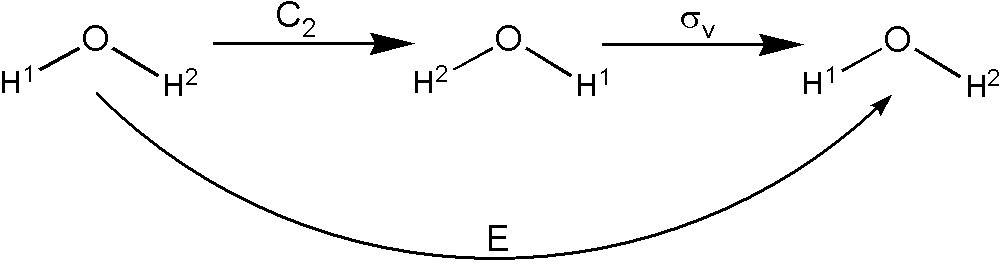
\includegraphics[width=.9\textwidth]{../img/point-group.png}
	\end{figure}
	\vfill
}

\subsection{Bodové grupy symetrie}
\frame{
	\frametitle{}
	\vfill
	\begin{itemize}
	\item Množina prvků symetrie, jejichž operace ponechávají alespoň jeden bod tělesa nepohyblivý.
	\item Příslušnost molekuly k bodové grupě se určuje pomocí prvků symetrie dané molekuly.
	\item Bodové grupy se označují pomocí \emph{Schönfliesovy symboliky}.
	\end{itemize}
	\hrule
	\begin{itemize}
	\item $C_1$: tato grupa obsahuje pouze identitu, CHFClBr
	\item $C_i$: E, i. Např. FClHC-CHClF
	\item $C_s$: E, s. Např. \ce{CH2ClF}
	\item $C_n$: E, C$_n$; \ce{H2O2}
	\item $C_{nv}$: E, C$_n$, n $\sigma_v$; \ce{H2O}, \ce{NH3}
	\item $C_{nh}$: E, C$_n$, n $\sigma_h$; \ce{H3BO3}, \emph{trans}-1,2-dichlorethen
	\end{itemize}
	\vfill
}

\frame{
	\frametitle{}
	\begin{figure}
		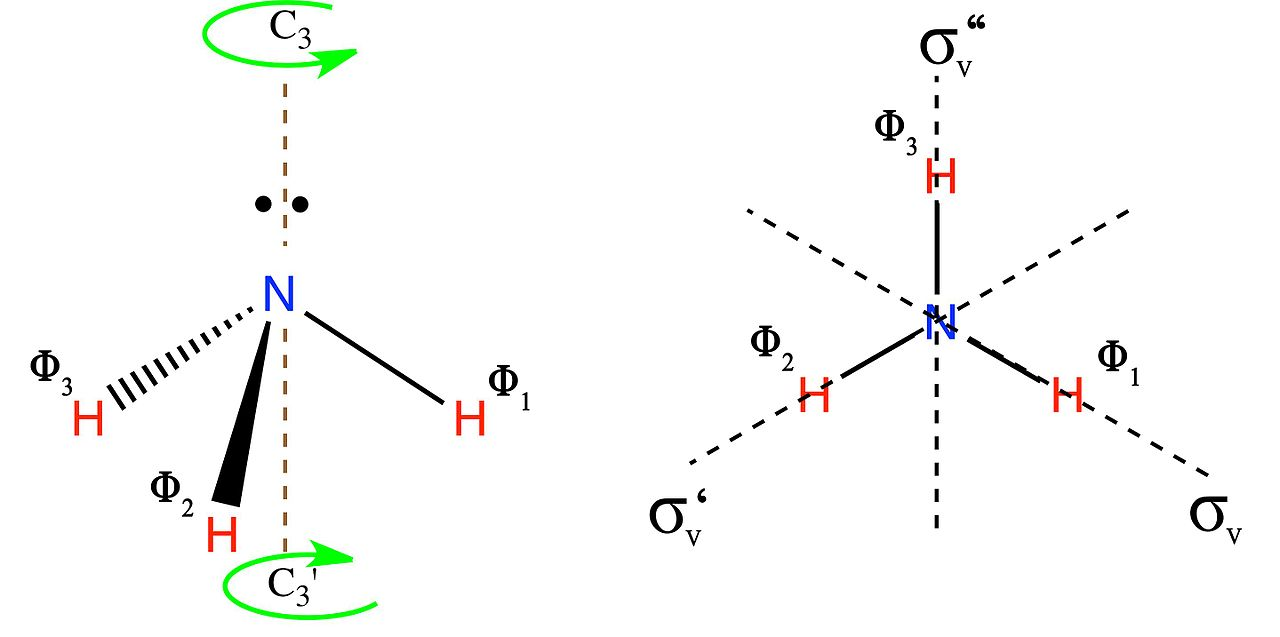
\includegraphics[width=0.95\textwidth]{../img/ammonia.jpg}
		\caption*{Operace symetrie v molekule amoniaku.\footnote[frame]{Zdroj: \href{https://commons.wikimedia.org/wiki/File:Defining_Each_Projection_Elements_.jpg}{Prasongm/Commons}}}
	\end{figure}
}

\frame{
	\frametitle{}
	\begin{figure}
		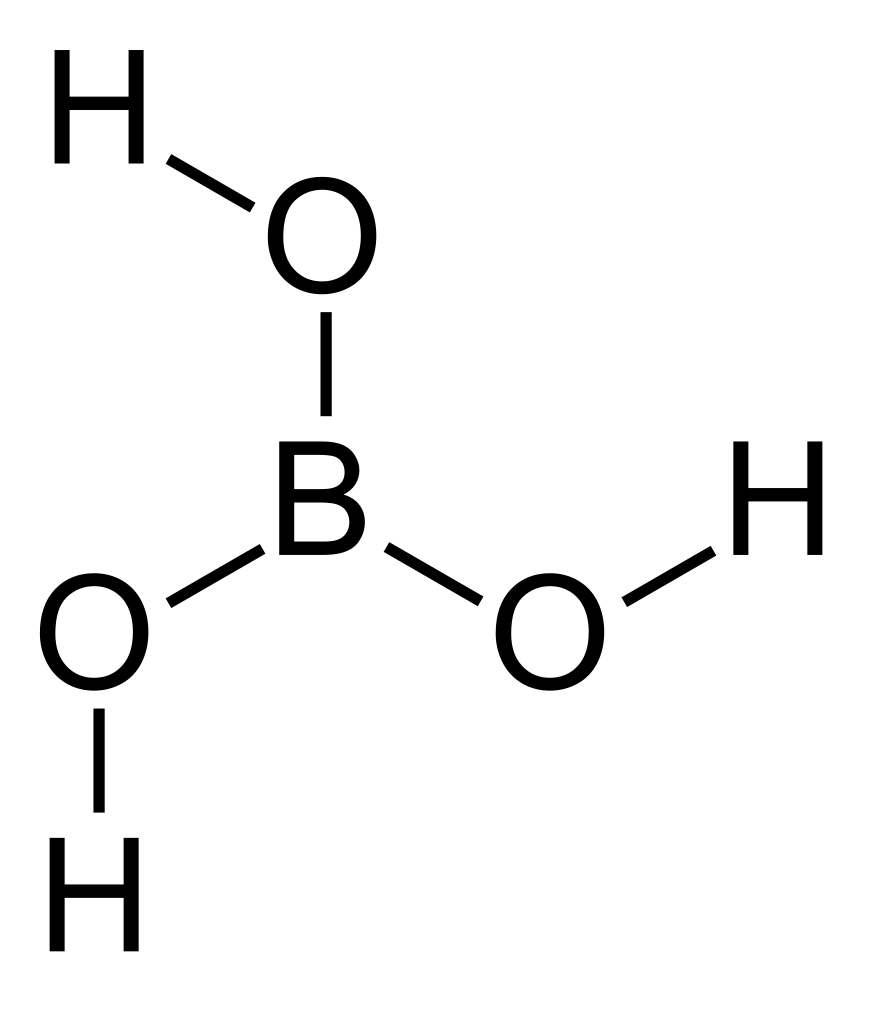
\includegraphics[width=0.5\textwidth]{../img/Boric-acid-2D.png}
	\end{figure}
}

\frame{
	\frametitle{}
	\begin{columns}[t]
	\column{.8\textwidth}
	\vfill
	\begin{itemize}
	\item $D_n$: E, C$_n$, n C$_2$; $D_1$ = $C_2$
	\item $D_{nh}$: E, C$_n$, n C$_2$, $\sigma_h$, pokud je n sudé, má grupa i střed symetrie; $D_{2h}$: naftalen; $D_{3h}$: \ce{BF3}
	\item $D_{nd}$: E, C$_n$, n C$_2$, $\sigma_d$, pokud je n liché, má grupa i střed symetrie
	\item \emph{Tetraedrické} - $T$, $T_d$, $T_h$
	\begin{itemize}
		\item $T_d$: E, 4 C$_3$, 3 C$_2$, 6 $\sigma_d$
		\item \ce{CH4}, \ce{SO4^{2-}}
	\end{itemize}
	\item \emph{Oktaedrické} - $O$, $O_h$
	\begin{itemize}
		\item $O_h$: E, 3 S$_4$, 3 C$_4$, 6 C$_2$, 4 S$_6$, 4 C$_3$, 3 $\sigma_h$, 6 $\sigma_d$, i
		\item \ce{SbF6}, \ce{Mo(CO)6}
	\end{itemize}
	\item \emph{Ikosaedrická} -$I_h$
	\begin{itemize}
		\item $I_h$: E, 6 S$_{10}$, 10 S$_6$, 6 C$_5$, 10 C$_3$, 15 C$_2$ and 15 $\sigma$
		\item \ce{B12}, \ce{C60}
	\end{itemize}
	\end{itemize}
	\vfill
	\column{.2\textwidth}
	\begin{center}
	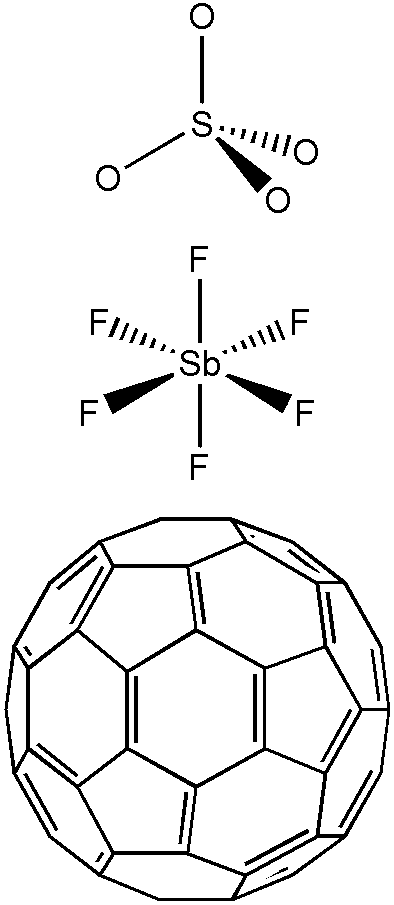
\includegraphics[width=25mm]{../img/cubic-point-groups.png}
	\end{center}
	\end{columns}

}

\frame{
	\frametitle{}
	\textbf{Dihedrální bodové grupy symetrie}
	\begin{itemize}
		\item Značí se D$_{nh}$.
		\item Obsahují E, C$_n$, n C$_2$ a $\sigma_h$
	\end{itemize}
	\begin{figure}
		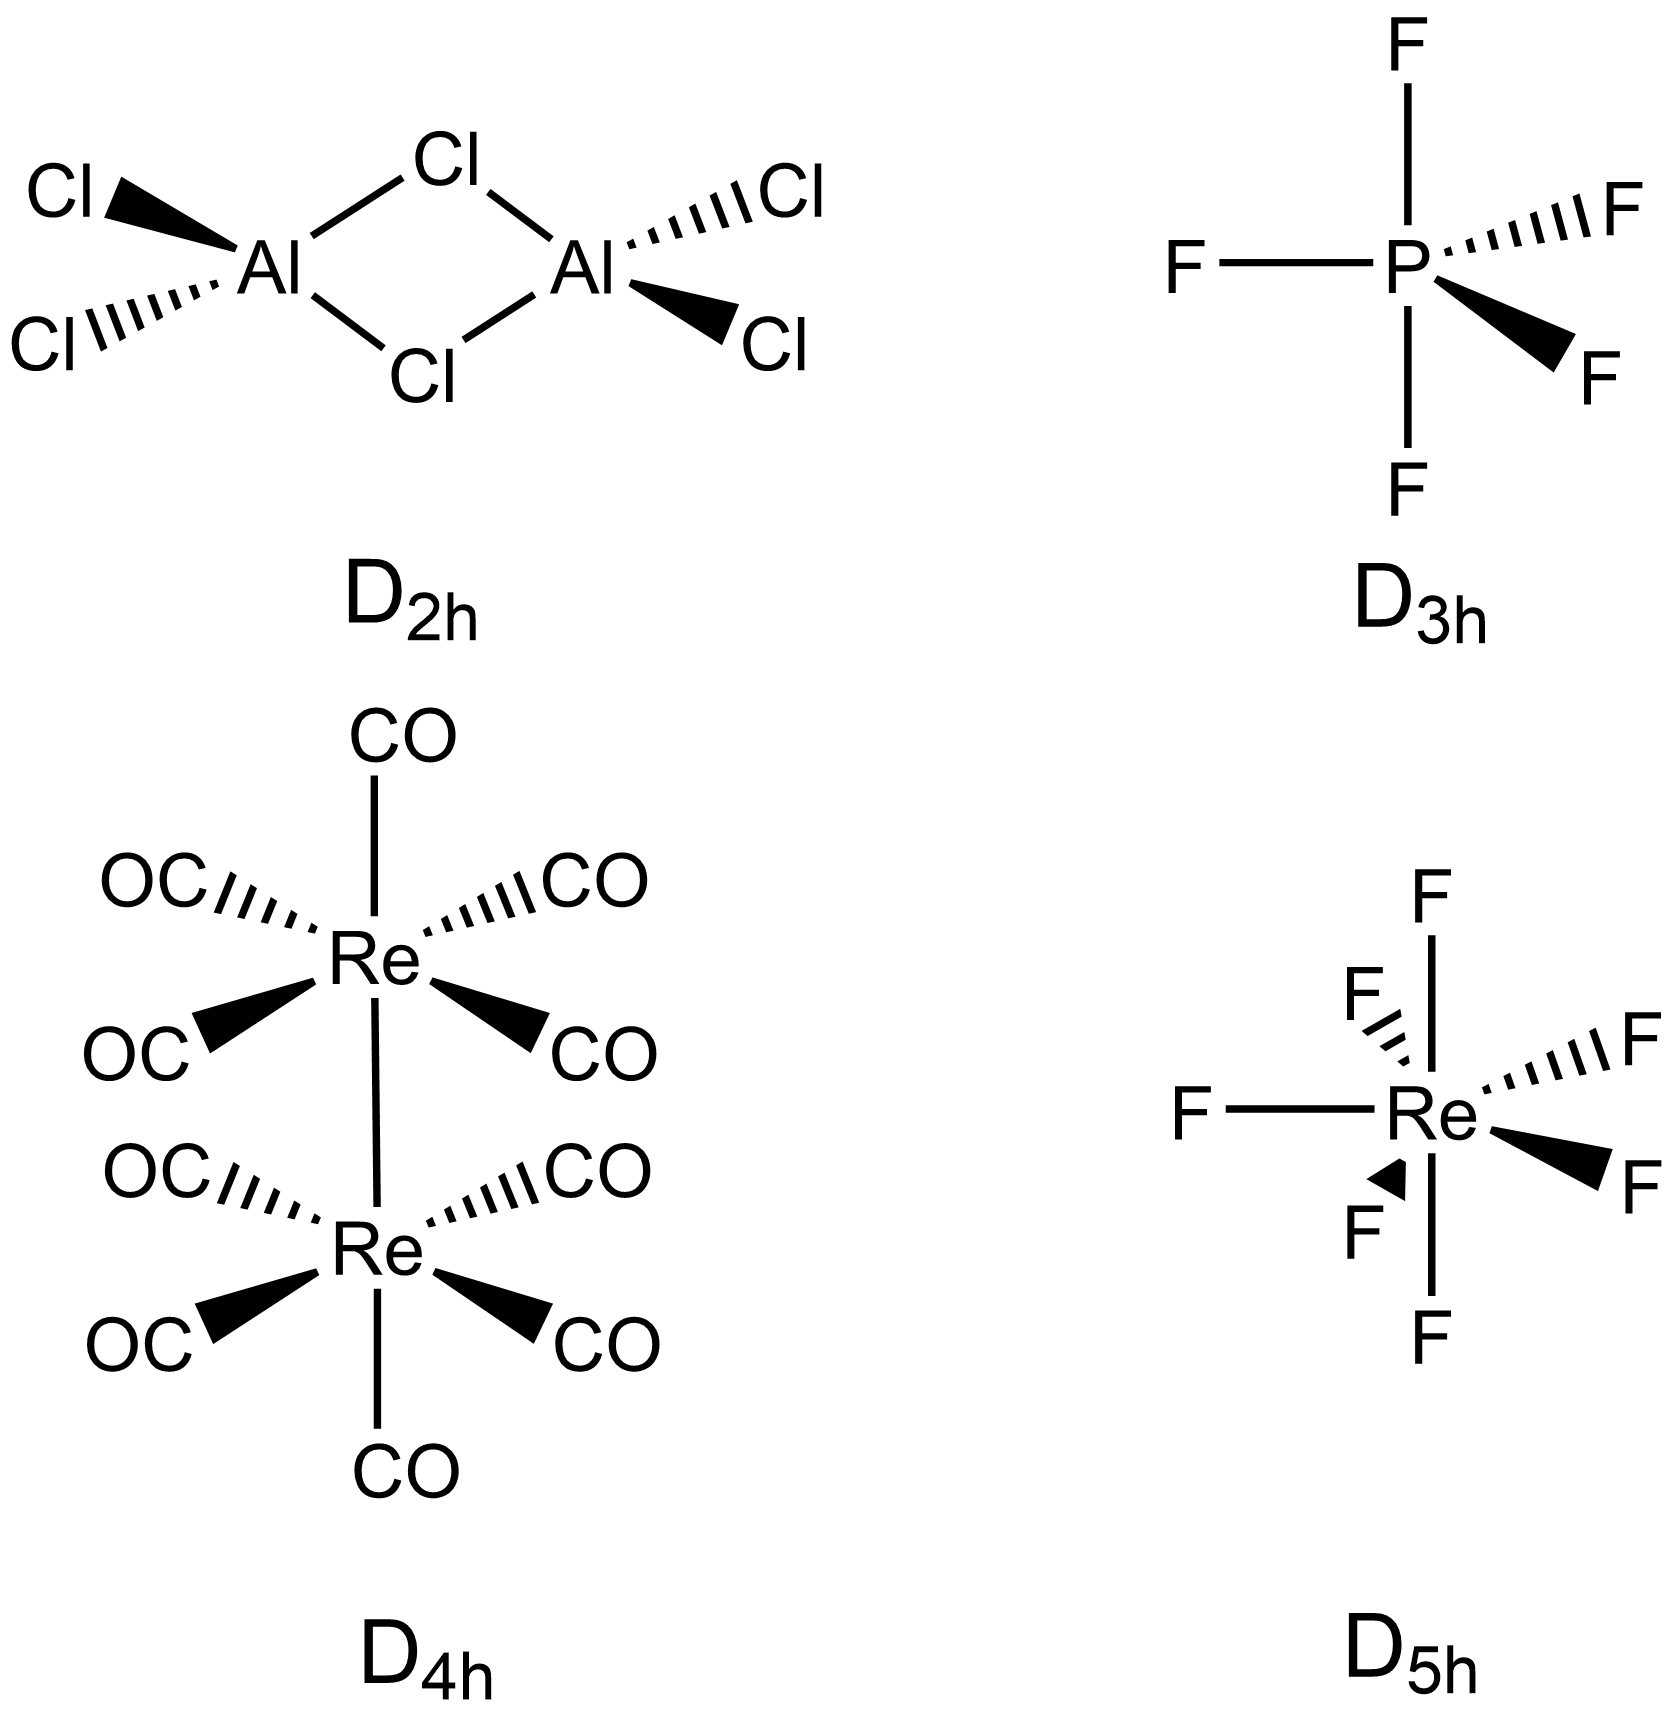
\includegraphics[width=0.6\textheight]{../img/Dnh.png}
	\end{figure}
}

\frame{
	\frametitle{}
	\begin{figure}
		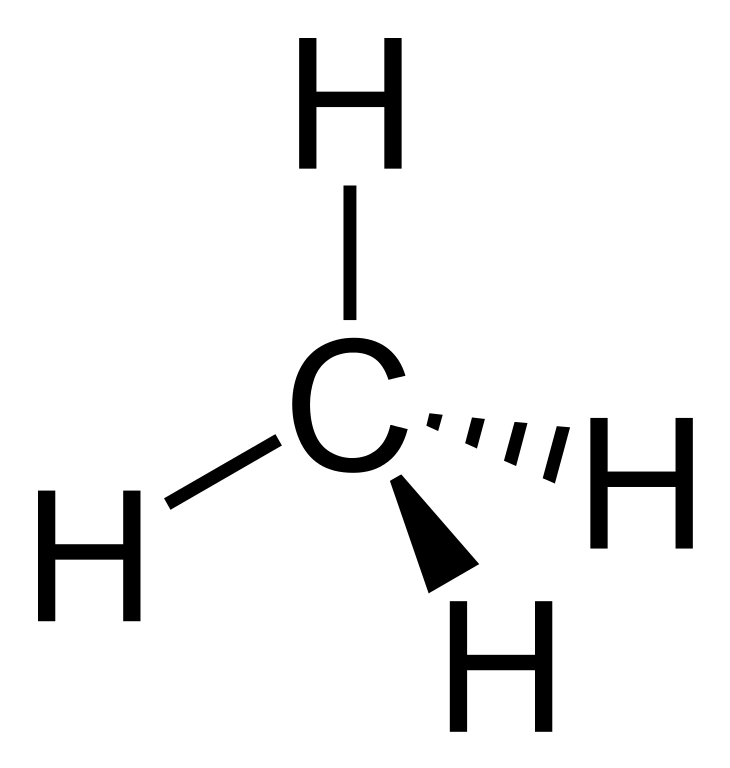
\includegraphics[width=0.6\textwidth]{../img/Methan.png}
	\end{figure}
}

\frame{
	\frametitle{}
	\begin{figure}
		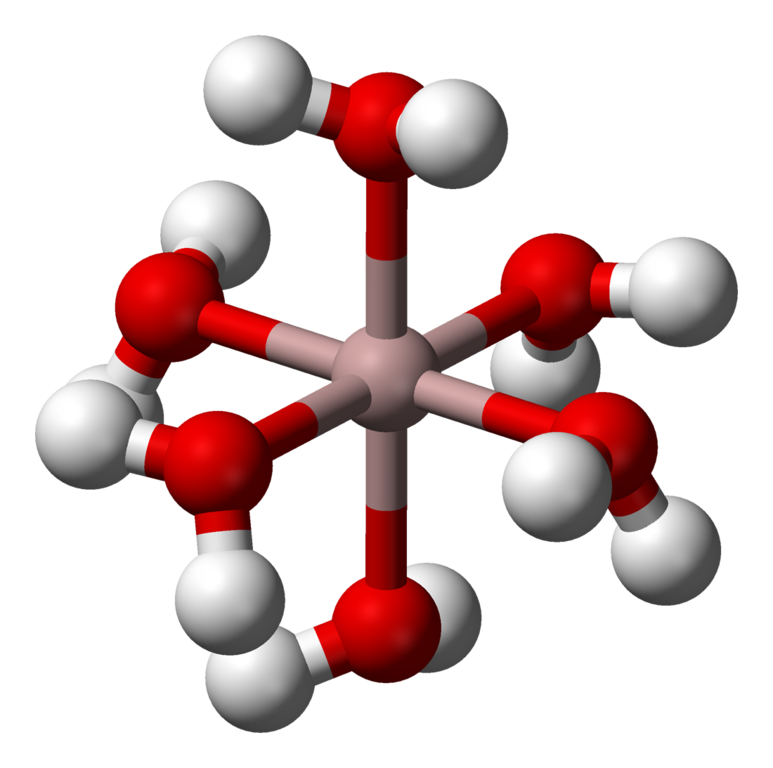
\includegraphics[width=0.55\textwidth]{../img/Al-H2O.png}
		\caption*{Kation \ce{[Al(H2O)6]3+}}
	\end{figure}
}

\frame{
	\frametitle{}
	\vfill
	\begin{itemize}
	\item \emph{Úplná rotační grupa} -$R_h$ - Obsahuje nekonečně mnoho os se všemi možnými hodnotami četnosti. Osy se protínají ve středu symetrie. Dále obsahuje nekonečně mnoho rovin symetrie, které procházejí středem symetrie.
	\end{itemize}
	\begin{center}
	
\includegraphics[width=5cm]{../img/spherical.png}
	\end{center}
	\vfill
}

\subsection{Dipólový moment}
\frame{
	\frametitle{}
	\vfill
	\begin{itemize}
	\item Vektor popisující rozložení elektrického náboje v molekule.
	\item Výsledný dipólmoment získáme vektorovým součtem dipólmomentů jednotlivých vazeb.
	\end{itemize}

	\begin{figure}
		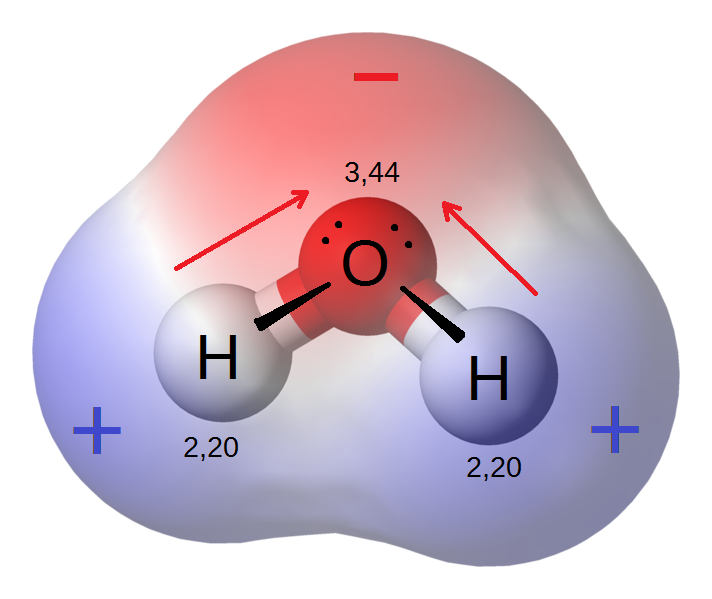
\includegraphics[width=5cm]{../img/Dipoli_acqua.png}
		\caption*{Dipólový moment molekuly vody.\footnote[frame]{Zdroj: \href{https://commons.wikimedia.org/wiki/File:Dipoli_acqua.png}{Riccardo Rovinetti/Commons}}}
	\end{figure}
	\vfill
}

\subsection{Absorpce infračerveného záření}
\frame{
	\frametitle{}
	\vfill
	\begin{itemize}
	\item Aby mohla molekula absorbovat infračervené záření musí během vibrace docházet ke změně dipólového momentu.
	\item Při absorpci dochází ke změně amplitudy vibrace, frekvence zůstává nezměněna.
	\item Intenzita absorpčních pásu je úměrná druhé mocnině změny dipólového momentu.
	\item Absorpcí infračerveného záření molekulami vznikají pásová spektra.
	\end{itemize}
	\vfill
}

\subsection{Infračervená spektroskopie}
\frame{
	\frametitle{}
	\vfill
	\begin{itemize}
	\item  NIR (0,7 -- 2,5 $\mu$m; 14 000 - 4 000 cm$^{-1}$) - infračervená spektroskopie v blízké oblasti
	\item  MIR (2,5 -- 25 $\mu$m; 4 000 - 400 cm$^{-1}$) - infračervená spektroskopie ve střední oblasti
	\item  FIR (25 -- 1000 $\mu$m; 400 - 10 cm$^{-1}$) - infračervená spektroskopie ve vzdálené oblasti
	\end{itemize}
	\vfill
}

\subsection{Absorpční spektrum}
\frame{
	\frametitle{}
	\vfill
	\adjincludegraphics[width=300pt,valign=l]{../img/spectrum.png}
	\begin{textblock*}{1cm}[1,1](55mm,65mm)
	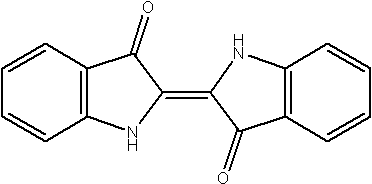
\includegraphics[width=80pt]{../img/spectrum-struct.png}
	\end{textblock*}
	\begin{itemize}
	\item Absorpční spektrum indiga
	\end{itemize}
	\vfill
}

\subsection{Měřící techniky}
\frame{
	\frametitle{}
	\vfill
	\begin{itemize}
	\item  FT-IR - transmise, ATR
	\item  DRIFT, IRRAS
	\item TG-IR, GC-IR
	\end{itemize}
	\vfill
}

\section{Infračervený spektrometr}
\frame{
	\frametitle{}
	\vfill
	\begin{itemize}
	\item Disperzní – za vzorkem je umístěn monochromátor (mřížka), který postupně propouští jednotlivé vlnové délky na detektor.
	\item Nedisperzní – využívá monochromatické zdroje záření.
	\item Interferometrický spektrometr (FT-IR)
	\begin{itemize}
	\item neobsahuje monochromátor, ale interferometr (Michelsonův interferometr)
	\item celé spektrum se snímá najednou a získaný interferogram je nutné zpracovat pomocí Fourierovy transformace.
	\item je citlivější než jiné typy spektrometrů.
	\end{itemize}
	\end{itemize}
	\vfill
}

\subsection{Zdroj infračerveného záření}
\frame{
	\frametitle{}
	\vfill
	\begin{columns}
		\begin{column}{.7\textwidth}
			\begin{itemize}
				\item \emph{Nernstova lampa} – lampa s žhavenou keramickou tyčinkou
				\item \emph{Globar}
				\begin{itemize}
					\item tyčinka z karbidu křemíku (SiC) vyhřívaná na teplotu 1000-1400 \textdegree C.
					\item keramická tyčinka omotaná odporovým drátem
				\end{itemize}
				\item \emph{IR LED} – diody z III/V polovodičů, poskytují monochromatické záření.
				\item \emph{IR lasery} – plynové nebo pevnolátkové lasery, zdroje monochromatického záření.
				\item \textit{QCL -- Quantum Cascade Laser} -- polovodičové lasery.
				\item \textit{Výbojky Hg-Ar} nebo \textit{Hg-Ne} se využívají pro oblast NIR.
			\end{itemize}
		\end{column}
		\begin{column}{.3\textwidth}
			\begin{figure}
				\adjincludegraphics[width=\textwidth]{../img/globar.jpg}
				\caption*{Nový a použitý globar}
			\end{figure}
		\end{column}
	\end{columns}
	\vfill
}

\subsection{Michelsonův interferometr}
\frame{
	\frametitle{}
	\vfill
	\begin{columns}
		\begin{column}{.7\textwidth}
			\begin{itemize}
				\item Autorem je americký fyzik Albert A. Michelson.
				\item Skládá se z beamsplitteru a dvou zrcadel.\footnote[frame]{\url{http://hyperphysics.phy-astr.gsu.edu/hbase/phyopt/michel.html}}
				\item Jedno ze zrcadel se pohybuje konstantní rychlostí po dráze kolmé k jeho ploše.
				\item Interferometr moduluje vstupující záření plynulou změnou rozdílu délky drah paprsků.\footnote[frame]{\href{https://www.youtube.com/watch?v=UA1qG7Fjc2A}{Interferometer -- animation}}
				\item Firma Bruker využívá interferometry s koutovými odražeči, tzv. RockSolid\texttrademark interferometry.\footnote[frame]{\href{http://bc.orgchm.bas.bg/~irlab/Site_BG/Laboratory/rocksolid.pdf}{The Bruker ROCKSOLID\texttrademark Interferometer}}
			\end{itemize}
		\end{column}
		\begin{column}{.3\textwidth}
			\begin{figure}
				\adjincludegraphics[width=\textwidth]{../img/Michelson_Interferometer.jpg}
				\caption*{Michelsonův interferometr.\footnote[frame]{Zdroj: \href{https://commons.wikimedia.org/wiki/File:Michelson_Interferometer.jpg}{Falcorian/Commons}}}
			\end{figure}
		\end{column}
	\end{columns}
	\vfill
}

\frame{
	\frametitle{}
	\vfill

Beamsplitter (BS) rozděluje paprsek ze zdroje na dva stejné paprsky. Jeden je odražen na nepohyblivé zrcadlo (Z1), od kterého se odrazí zpět. Druhý projde beamsplitterem a dopadne na pohyblivé zdrcadlo (Z2). Oba paprsky dopadnou zpět na BS, kde interferují a výsledný paprsek je znovu zčásti odražen k detektoru a z části projde BS směrem ke zdroji. Intenzita výsledného paprsku je závislá na rozdílu vzdáleností obou zrcadel od BS.

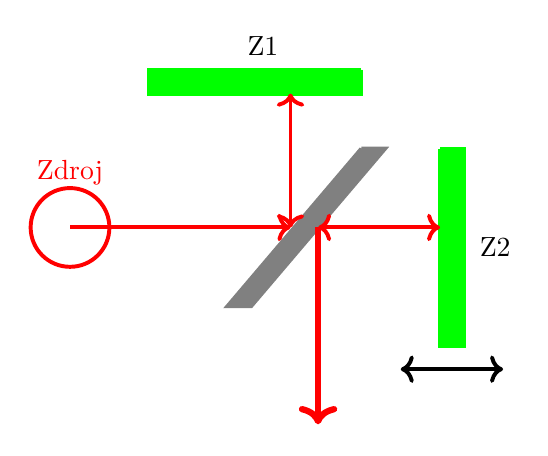
\begin{tikzpicture}
\draw[line width=0.5mm, red] (2,1) circle (0.5);
\node[red] at (2,1.7) {Zdroj};
\node at (4.45,3.3) {Z1};
\node at (7.4,0.75) {Z2};

\draw[line width=0.5mm,gray,fill=gray] (5.7,2) -- (6,2) -- (4.3,0) -- (4,0) -- (5.7,2);

\draw[line width=0.5mm,green,fill=green] (5.7,3) -- (5.7,2.7) -- (3,2.7) -- (3,3) -- (5.7,3);
\draw[line width=0.5mm,green,fill=green] (6.7,2) -- (7,2) -- (7,-0.5) -- (6.7,-0.5) -- (6.7,2);
\draw[line width=0.5mm,black,<->] (6.2,-0.8) -- (7.5,-0.8);

\draw[line width=0.5mm,red,->] (2,1) -- (4.8,1);
\draw[line width=0.5mm,red,<->] (4.8,2.7) -- (4.8,1);
\draw[line width=0.5mm,red,<->] (6.7,1) -- (5.15,1);

\draw[line width=0.8mm,red,->] (5.15,1) -- (5.15,-1.5);

\end{tikzpicture}
	\vfill
}

\subsection{Detektory}
\frame{
	\frametitle{}
	\vfill
	\begin{columns}
		\begin{column}{.6\textwidth}
			Nejčastěji se využívají pyroelektrické detektory.
			\begin{itemize}
				\item \emph{DLaTGS}
				\begin{itemize}
					\item triglycinsulfát dopovaný L-alaninem
					\item pyroelektrický detektor
				\end{itemize}
				\item \emph{MCT}
				\begin{itemize}
					\item mercury/cadmium/telluride
					\item fotovodivostní detektor (dioda)
					\item citlivější než DLaTGS
					\item vyžaduje chlazení na teplotu kapalného dusíku
				\end{itemize}
				\item \emph{TEC-MCT}
				\begin{itemize}
					\item ThermoElectrically Cooled MCT\footnote[frame]{\href{https://assets.thermofisher.com/TFS-Assets/CAD/Technical-Notes/thermoelectrically-mct-ftir-microscope-tn1036-en.pdf}{The Thermoelectrically cooled MCT (TEC-MCT) used in an FTIR microscope}}
				\end{itemize}
			\end{itemize}
		\end{column}
		\begin{column}{.3\textwidth}
			\begin{figure}
				\adjincludegraphics[height=.4\textheight]{../img/Pyroelectric-detector.jpg}
				\caption*{Pyroelektrický detektor.\footnote[frame]{Zdroj: \href{https://commons.wikimedia.org/wiki/File:Busch-Jaeger_Elektro_UP_Sensor_180_Komfort_6132_-_board_-_Heimann_LHI_958-0677.jpg}{Raimond Spekking/Commons}}}
			\end{figure}
		\end{column}
	\end{columns}
	\vfill
}

\frame{
	\frametitle{}
	\vfill
	Pro oblast NIR se využívají detektory InGaAs nebo chlazené CCD čipy.
	\begin{itemize}
		\item \emph{InGaAs}
		\begin{itemize}
			\item Ternární slitina arsenidu gallitého (GaAs) a inditého (InAs).
			\item III-V polovodič.
		\end{itemize}
		\item \textit{CCD} - \textbf{C}harge \textbf{C}oupled \textbf{D}evice
		\begin{itemize}
			\item Vícekanálový detektor (Multi-channel).
			\item Pro zvýšení citlivosti (snížení šumu) pracuje za teploty kapalného dusíku nebo využívá chlazení pomocí Peltierových článků.
			\item Parametry CCD (velikost pixelu) určují rozlišení naměřeného spektra.
		\end{itemize}
	\end{itemize}
	\begin{figure}
		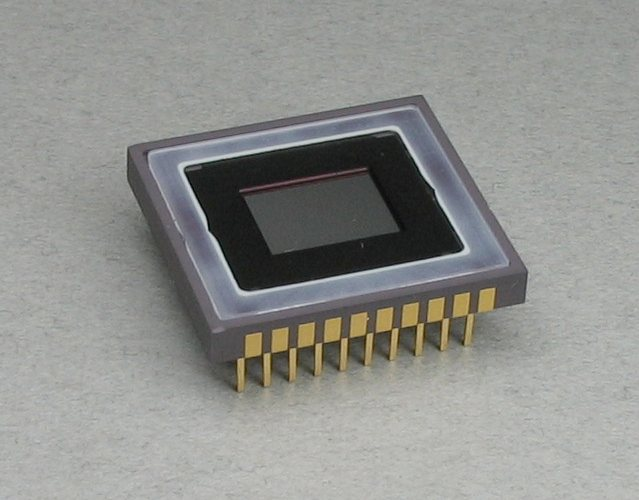
\includegraphics[height=.15\textheight]{../img/CCD.jpg}
		\caption*{CCD čip\footnote[frame]{Zdroj: \href{https://commons.wikimedia.org/wiki/File:Pmside2.jpg}{Sphl/Commons}}}
	\end{figure}
	\vfill
}

\section{Měřící techniky}
\subsection{FT-IR}
\frame{
	\frametitle{}
	\vfill
	\begin{itemize}
	\item  Nejběžnější měřící technika
	\item Podle úpravy vzorku rozlišujeme měření v transmisním módu a ATR
	\item Spektrometr neobsahuje monochromátor, ale interferometr
	\item Celé spektrum se snímá najednou, získáme interferogram, který je nutné zpracovat pomocí Fourierovy transformace
	\end{itemize}
	\vfill
}

\frame{
	\frametitle{}
	\vfill
	\begin{figure}
		\adjincludegraphics[width=.8\textwidth]{../img/ftir.png}
		\caption*{Schéma FT-IR spektrometru.\footnote[frame]{Zdroj: \href{https://commons.wikimedia.org/w/index.php?lang=cs&title=File\%3AFourier_Transform_spectrometer_principle.svg}{Joachim Terschluesen/Commons}}}
	\end{figure}
	\vfill
}

\frame{
	\frametitle{}
	\vfill
	\adjincludegraphics[width=11cm,valign=l]{../img/tensor.png}
	\vfill
}

\subsection{Transmisní měření}
\frame{
	\frametitle{}
	\vfill
	\begin{itemize}
	\item  Lze měřit pevné látky, kapaliny i plyny
	\item Pevné látky měříme ve formě KBr tablet (1-3 hm. \% v KBr) nebo jako suspenze v Nujolu
	\item Kapaliny měříme jako tenký film mezi okny z vhodného materiálu (KBr, KRS, NaCl, ...)
	\end{itemize}
	\adjincludegraphics[width=300pt,valign=l]{../img/kbr-pellets.png}
	\vfill
}

\subsection{Transmisní měření - Nujol}
\frame{
	\frametitle{}
	\vfill
	\begin{itemize}
	\item Nujol - směs alkanů s dlouhý řetězcem.
	\end{itemize}
	\adjincludegraphics[width=300pt,valign=l]{../img/nujol.png}
	\vfill
}

\subsection{Transmisní měření - plynné vzorky}
\frame{
	\frametitle{}
	\vfill
	\begin{itemize}
	\item Plyny se měří v plynových kyvetách, ty jsou konstruované tak, aby dráha paprsku byla co nejdelší
	\item Protože v plynném skupenství existují pouze slabé interakce mezi částicemi lze naměřit čistě rotační i rotačně-vibrační spektra
	\end{itemize}
	\adjincludegraphics[width=90mm,valign=l]{../img/water.png}
	\vfill
}

\frame{
	\frametitle{}
	\vfill
	\begin{figure}
		\adjincludegraphics[width=0.4\textwidth]{../img/IFS-125HR.jpg}
	\end{figure}
	\vfill
}

\subsection{ATR}
\frame{
	\frametitle{}
	\vfill
	\begin{itemize}
	\item ATR - Attenuated Total Reflection\footnote[frame]{Zeslabený úplný odraz}
	\item Krystaly jsou z diamantu, ZnSe, Ge, KRS-5 (směs TlBr a TlI) nebo křemíku
	\item Vzorek se přitlačí vysokým tlakem k měřícímu krystalu, dochází k úplnému odrazu\footnote[frame]{\href{https://www.youtube.com/watch?v=O4kujZQ8YgA}{Optické kabely – Tomáš Tyc}}
	\item Paprsek se pohybuje po povrchu vzorku (0,5 - 5 $\mu$m)
	\end{itemize}
	\vfill
	\begin{figure}
		\adjincludegraphics[width=.8\textwidth]{../img/ATR.png}
		\caption*{Schéma ATR.\footnote[frame]{Zdroj: \href{https://commons.wikimedia.org/wiki/File:ATR_path-en.svg}{Fulvio314/Commons}}}
	\end{figure}
}

\frame{
	\frametitle{}
	\vfill
	\begin{figure}
		\adjincludegraphics[height=0.6\textheight]{../img/tensor-atr.png}
		\caption*{ATR nástavec, spektrometr Bruker Tensor 27}
	\end{figure}
	\vfill
}

\frame{
	\frametitle{}
	\vfill
	\begin{center}
		\begin{tabular}{|p{3cm}|c|p{5cm}|}
			\hline
			Materiál krystalu & Index lomu & Použití \\
			\hline
			Germanium & 4 & Vhodné pro většinu vzorků. \\
			\hline
			Křemík & 3,4 & Odolný vůči zásaditým roztokům. \\
			\hline
			AMTIR (speciální skla pro IR) & 2,5 & Odolné vůči kyselým roztoků \\
			\hline
			ZnSe & 2,4 & Vhodné pro většinu vzorků. \\
			\hline
			Diamant & 2,4 & Vhodné pro většinu vzorků, i pro velmi tvrdé nebo agresivní látky. \\
			\hline
		\end{tabular}
	\end{center}
	\vfill
}

\frame{
	\frametitle{}
	\vfill
	\begin{itemize}
		\item \textit{BioATR} - speciální cely umožňující ATR-IR měření biologických vzorků.
		\item Mají malý objem a vzorky je možné temperovat.
		\item Umožňují stanovení teploty, při které dochází ke konformační změně proteinů.
		\item Lze měřit jak statické vzorky, tak i v módu průtočné kyvety.
	\end{itemize}
	\vfill
}

\subsection{FPA}
\frame{
	\frametitle{}
	\vfill
	\begin{itemize}
		\item FPA - Focal Plane Array detector
		\item Plošný detektor, umožňuje mikroskopickou analýzu větších vzorků, např. vzorků mikroplastů.\footnote[frame]{\href{https://chemagazin.cz/archiv-casopisu/chemagazin-3-2024-plyny}{Mikroplasty pod mikroskopem: využití perspektivní FTIR-FPA technologie v praxi. Chemagazín 2024/3}}
	\end{itemize}
	\vfill
	\begin{figure}
		\adjincludegraphics[height=.4\textheight]{../img/Webb_Instruments_Perfected_to_Microscopic_Levels.jpg}
		\caption*{FPA NIR detektor z JWST.\footnote[frame]{Zdroj: \href{https://commons.wikimedia.org/wiki/File:Webb_Instruments_Perfected_to_Microscopic_Levels_(14486243743).jpg}{NASA/Commons}}}
	\end{figure}
}

\subsection{IRRAS}
\frame{
	\frametitle{}
	\vfill
	\begin{itemize}
	\item IRRAS - IR Reflection Absorption Spectroscopy
	\item Metoda vhodná pro tenké vrstvy nanesené na kovových materiálech nebo nasorbované látky na materiálech
	\item Pro zvýšení citlivosti se využívá polarizovaného záření
	\end{itemize}
	\begin{figure}
		\adjincludegraphics[width=.8\textwidth]{../img/irras.png}
		\caption*{Blokové schéma IRRAS. A: zdroj IR záření; B: polarizátor; C: fázový modulátor; D: vzorek; E: detektor\footnote[frame]{Zdroj: \href{https://commons.wikimedia.org/wiki/File:Principe_PM-IRRAS.png}{Steff-X/Commons}}}
	\end{figure}
	\vfill
}

\subsection{DRIFTS, PAS}
\frame{
	\frametitle{}
	\vfill
	\begin{itemize}
	\item \textbf{DRIFTS}
	\begin{itemize}
		\item Diffuse Reflectance Infrared Fourier Transform Spectroscopy\footnote[frame]{\href{https://www.youtube.com/watch?v=83S6IIWNeBE}{Diffuse Reflection Reaction Monitoring}}
		\item Tato technika je vhodná pro měření malých částic nebo hrubých povrchů
		\item Využívá rozptylu IR záření
		\item Rozptýlené záření je pomocí kulového zrcadla odráženo na detektor
		\item Práškové vzorky se měří v kelímcích, pevné vzorky se obrousí abrasivem (SiC) a měří se částice zachycené na abrasivu
	\end{itemize}
	\item \textbf{FTIR-PAS}
	\begin{itemize}
		\item Photoacoustic Fourier Transform Infrared Spectroscopy - kombinace FTIR a fotoakustické spektroskopie.
		\item Absorpci modulovaného záření vede k lokálnímu zahřátí absorbujícího objemového prvku. Vzniklé tlakové vlny jsou detekovány citlivým tlakovým detektorem, který vytváří signál úměrný absorpci.
		\item Výhodné pro měření plynů, protože vzorkovací prostor může být velmi malý.
	\end{itemize}
	\end{itemize}
	\vfill
}

\subsection{AFM-ATR}
\frame{
	\frametitle{}
	\vfill
	\begin{columns}
		\begin{column}{.5\textwidth}
			\begin{itemize}
				\item AFM -- Atomic Force Microscopy.
				\item Obraz vzorku je snímám pomocí interakce velmi tenkého hrotu s povrchem vzorku.
				\item Hrot AFM se využívá i k detekci IR spektra.
				\item Zdrojem záření je QCL\footnote[frame]{\href{https://spie.org/publications/spie-publication-resources/optipedia-free-optics-information/fg12_p45_quantum_cascade_lasers}{QCL -- Quantum Cascade Lasers}}, při absorpci dojde ke zvýšení teploty v místě dopadu.
				\item Můžeme mapovat rozložení látek ve vzorku s rozlišením daným AFM.
			\end{itemize}
		\end{column}

		\begin{column}{.5\textwidth}
			\begin{figure}
				\adjincludegraphics[width=\textwidth]{../img/AFMsetup.jpg}
				\caption*{Schéma AFM.\footnote[frame]{Zdroj: \href{https://commons.wikimedia.org/wiki/File:AFMsetup.jpg}{KristianMolhave/Commons}}}
			\end{figure}
		\end{column}
	\end{columns}
	\vfill
}

\frame{
	\frametitle{}
	\vfill
	\begin{figure}
		\adjincludegraphics[height=.67\textheight]{../img/AFM_3D_Topography.jpg}
		\caption*{AFM snímek nanočástic palladia.\footnote[frame]{Zdroj: \href{https://commons.wikimedia.org/wiki/File:AFM_3D_Topography_Image_of_Palladium_Nanoparticles_on_Chitosan_Film.tif}{Mehrabanian/Commons}}}
	\end{figure}
	\vfill
}

\subsection{Coupling TGA/IR}
\frame{
	\frametitle{}
	\vfill
	\begin{itemize}
	\item TGA - termogravimetrická analýza
	\item Plyny vznikající během degradace vzorku vedeme do měřící cely a pomocí IR spektroskopie stanovíme jejich složení
	\item Během transportu plynů z pece do měřící cely dochází k velkému zředění plynu, proto je nutné používat citlivější detektory (MCT)
	\end{itemize}
	\begin{figure}
		\adjincludegraphics[width=.75\textwidth]{../img/tg-irFoto.jpg}
	\end{figure}
	\vfill
}

\frame{
	\frametitle{}
	\vfill
	\begin{figure}
		\adjincludegraphics[width=.75\textwidth]{../img/tg-ir.png}
	\end{figure}
	\vfill
}

\subsection{Coupling GC/IR}
\frame{
	\frametitle{}
	\vfill
	\begin{itemize}
	\item GC - plynová chromatografie
	\item Méně citlivé než GC/MS, ale umožňuje analýzu stereoizomerů.
	\item Interferogramy je nutné snímat v krátkých časových intervalech
	\end{itemize}
	\adjincludegraphics[width=10cm,valign=l]{../img/gc-ir.jpg}
	\vfill
}

\section{Kvantitativní analýza}
\frame{
	\frametitle{}
	\vfill
	\begin{itemize}
	\item \emph{Lambert-Beerův zákon} -- $A_\lambda = \epsilon_\lambda l c$
	\begin{itemize}
		\item $A_\lambda$ - absorbance vzorku při vlnové délce $\lambda$
		\item $\epsilon_\lambda$ - absorpční koeficient při vlnové délce $\lambda$. Je charakteristický pro každou sloučeninu.
		\item l - délka kyvety
		\item c - koncentrace vzorku
	\end{itemize}
	\item Pro stanovení koncentrace se využívá \emph{kalibrační křivka}.
	\end{itemize}
	\vfill
}

\section{Využití IR spektroskopie}
\subsection{Chemie}
\frame{
	\frametitle{}
	\vfill
	\begin{itemize}
	\item Identifikace sloučenin srovnáním spekter s databází
	\item Kontrola čistoty připravených produktů, výhodou metody je její vysoká citlivost
	\item Kvalitativní a kvantitativní analýza polymerů, analýza degradačních produktů
	\item Monitorování polymerizačních reakcí
	\item Analýza povrchových vrstev s využitím ATR
	\item Kvantitativní analýza - Lambert-Beerův zákon:
	\begin{itemize}
		\item Plyny: \scalebox{1.2}{$A=\frac{p \epsilon l}{RT}$}
		\item Kapaliny: $A=\epsilon cl$
		\item Je nutné zvolit vhodný pás - vysoký absorpční koeficient, bez překryvu s okolními pásy, symetrický a vykazující lineární závislost intenzity na koncentraci
	\end{itemize}
	\end{itemize}
	\vfill
}

\subsection{Restaurování a konzervování uměleckých děl}
\frame{
	\frametitle{}
	\vfill
	\begin{itemize}
	\item Výhodou IR spektroskopie je nízká spotřeba vzorku, příp. nedestruktivnost metody, při použití bezkontaktního spektrometru.\footnote[frame]{\href{https://www.azom.com/article.aspx?ArticleID=15230}{Contactless Analysis of Paintings with FTIR Spectroscopy}}
	\end{itemize}
	\adjincludegraphics[scale=0.4]{../img/nova-contactless.png}
	\vfill
}

\frame{
	\frametitle{}
	\vfill
	\begin{itemize}
	\item Rutinně lze provést analýzy pigmentů, pojiv, organických složek (dřevěné rámy, povrchové úpravy, apod.)
	\item Mezi speciální aplikace patří např. datování dřeva, které může být pro mladší dřevěné předměty podstatně přesnější než datování pomocí $^{14}C$.
	\item FT-IR mikroskop se lze využít k analýze nábrusů a identifikaci složení a stratigrafie vrstev
	\end{itemize}
	\adjincludegraphics[scale=0.7]{../img/mikroskop.jpg}
	\vfill
}

\subsection{Analýza potravin}
\frame{
	\frametitle{}
	\vfill
	\begin{columns}
		\begin{column}{.58\textwidth}
			\begin{itemize}
				\item FT-NIR je velmi výhodná metoda pro analýzu potravin.
				\item Je velmi rychlá, levná, nedestruktivní a bezpečná.
				\item Vzorky není nutné upravovat, lze měřit přímo v baleních.
				\item Kapaliny je možné analyzovat pomocí průtočné měřící cely.
				\item Umožňuje snadnou analýzu vstupních surovin, meziproduktů i finálních výrobků.
			\end{itemize}
		\end{column}
		\begin{column}{.45\textwidth}
			\begin{figure}
				\adjincludegraphics[width=\textwidth]{../img/NIR-melanine.jpg}
				\caption*{Analýza laktózy pomocí NIR.\footnote[frame]{Zdroj: \href{https://commons.wikimedia.org/wiki/File:Portable_Screening_Devices_(1432)_(8225043720).jpg}{FDA/Commons}}}
			\end{figure}
		\end{column}
	\end{columns}
	\vfill
}

\subsection{Fluor v lyžařských voscích}
\frame{
	\frametitle{}
	\vfill
	\begin{columns}
		\begin{column}{.53\textwidth}
			\begin{itemize}
				\item Lyžařské vosky s obsahem PFAS jsou od sezóny 2023/2024 zakázány mezinárodní lyžařskou federací (FIS).\footnote[frame]{\href{https://www.seznamzpravy.cz/clanek/sport-stop-fluorovym-lyzarskym-voskum-funguji-skvele-ale-skodi-zdravi-228268}{Stop fluorovým lyžařským voskům. Fungují skvěle, ale škodí zdraví}}
				\item Důvodem je vysoká stabilita PFAS a jejich ukládání v životním prostředí.
				\item Jednou z možností, jak kontrolovat dodržování zákazu je IR spektroskopie.
			\end{itemize}
		\end{column}
		\begin{column}{.5\textwidth}
			\begin{figure}
				\adjincludegraphics[width=\textwidth]{../img/C-F-wax.jpg}
				\caption*{Vibrační pásy C-F v IR spektrech lyžařských vosků.\footnote[frame]{Zdroj: \href{https://doi.org/10.1016/j.coldregions.2024.104365}{Chemical composition and properties of Ski wax: A comprehensive analysis of fluorinated, non-fluorinated, and bio-based waxes}}}
			\end{figure}
		\end{column}
	\end{columns}
	\vfill
}

\subsection{Biologie}
\frame{
	\frametitle{}
	\vfill
	\begin{columns}
		\begin{column}{.63\textwidth}
			\begin{itemize}
				\item FTIR spektroskopii lze využít i ke studiu biologických systémů.
				\item Ve spektrech lze nalézt kvalitativní i kvantitativní informaci o chemickém složení.
				\item Kvantifikace se provádí na základě vhodných kalibračních modelů.
			\end{itemize}
		\end{column}
		\begin{column}{.4\textwidth}
			\begin{figure}
				\adjincludegraphics[width=\textwidth]{../img/FTIR-roots.jpg}
				\caption*{IR spektra kořenů z Finska.\footnote[frame]{Zdroj: \href{https://doi.org/10.3389/fpls.2020.00597}{Quantification of Plant Root Species Composition in Peatlands Using FTIR Spectroscopy}}}
			\end{figure}
		\end{column}
	\end{columns}
	\vfill
}

\frame{
	\frametitle{}
	\vfill
	\begin{itemize}
	\item IR spektrosokopii lze využít ke studiu biologických systémů, tzn. lipidů, proteinů, peptidů, biomembrán, nukleových kyselin, tkání, buněk, atd.
	\item U fosfolipidů lze stanovit konformaci řetězce a tím získat informace o uspořádání v buňce
	\item IR spektra proteinů obsahují výrazné absorpční pásy amidové skupiny, podle jejich vlnočtu a intenzity lze určit konformaci a sekundární strukturu (dekonvolucí a fitováním pásů)
	\end{itemize}
	\adjincludegraphics[scale=0.4]{../img//amide-IR.png}
	\vfill
}

\frame{
	\frametitle{}
	\vfill
	\begin{itemize}
	\item Spektra nukleových kyselin poskytují informace o konformaci hlavního řetězce kyseliny a o párování bází
	\item IR spektra lze využít i pro diagnostiku nádorů, např. sledováním závislosti polohy pásu deformační vibrace methylenové skupiny na tlaku lze odlišit zdravou a rakovinovou tkáň
	\end{itemize}
		\adjincludegraphics[scale=0.4]{../img//pressure-dependence.png}
	\vfill
}

\frame{
	\frametitle{}
	\vfill
	\begin{itemize}
		\item ATR techniku lze využít i pro monitorování struktury proteinů a jejich agregace.\footnote[frame]{\href{https://www.spectroscopyonline.com/view/atr-ft-ir-a-new-vision-on-protein-structure-and-aggregation}{ATR FT-IR: A New Vision on Protein Structure and Aggregation}}
		\item Studium oblasti 1700--1600 cm$^{-1}$ může pomoci s identifikací sekundární struktury proteinů, např. rozlišit šroubovici ($\alpha$-helix) a skládaný list.
	\end{itemize}
	\begin{figure}
		\adjincludegraphics[width=.35\textwidth]{../img/ATR-protein.jpg}
		\caption*{Měření ATR v průtokovém módu.\footnote[frame]{Zdroj: \href{https://doi.org/10.1016/j.saa.2023.123629}{ScienceDirect}}}
	\end{figure}
	\vfill
}

\end{document}